% TemplateV5.tex --  LaTeX-based template for submissions to the American Meteorological Society
% Version 5.0, 2 January 2020

% Paper layout
%\documentclass{ametsocV5} %for submission
\documentclass[twocol]{ametsocV5} % two-column layout (for author use only)

% Packages
\usepackage{amsmath,amsfonts,amssymb,bm}
\usepackage{mathptmx}
\usepackage{newtxtext}
\usepackage{newtxmath}
\usepackage{enumitem}
\usepackage{multirow}
\usepackage{amsmath}



%%%%%%%%%
% TITLE %
%%%%%%%%%
\title{Operational adoption of new probabilistic point rainfall forecasts: the crucial role of a user-centric training}


%%%%%%%%%%%
% AUTHORS %
%%%%%%%%%%%

\authors{Fatima M. Pillosu\correspondingauthor{Fatima Pillosu, fatima.pillosu@ecmwf.int}}
\affiliation{University of Reading, Reading, UK \\
European Centre for Medium-Range Weather Forecasts, Reading, UK}

\extraauthor{Boglárka Tóth, Istvan Ihasz}
\extraaffil{Hungarian Meteorological Service, Budapest, Hungary}

\extraauthor{Roberto Vindas Morán, Werner Stolz}
\extraaffil{National Meteorological Institute of Costa Rica, San José, Costa Rica}

\extraauthor{Tim Hewson}
\extraaffil{European Centre for Medium-Range Weather Forecasts, Reading, UK}

\extraauthor{Christel Prudhomme}
\extraaffil{European Centre for Medium-Range Weather Forecasts, Reading, UK \\
Loughborough University, Loughborough, UK}

\extraauthor{Elisabeth Stephens}
\extraaffil{University of Reading, Reading, UK}

\extraauthor{Hannah L. Cloke}
\extraaffil{University of Reading, Reading, UK \\
Uppsala University, Uppsala, Sweden \\
Centre of Natural hazards and Disaster Science, Uppsala, Sweden}



%%%%%%%%%%%%
% ABSTRACT %
%%%%%%%%%%%%



%%%%%%%%%%%%%%%%%%%%%%
% MAIN BODY OF PAPER %
%%%%%%%%%%%%%%%%%%%%%%
\begin{document}
\maketitle


%%%%%%%%%%%%%%%%%%%%
% INTRODUCTION
\section{Introduction}

Worldwide, extreme weather-related hazards (e.g. tropical cyclones, floods, landslides, droughts, heatwaves, wildfires, earthquakes, tsunamis, volcanoes) have cost millions of lives and billions of dollars in economic losses between 2000-2019 (UNDRR 2020). Moreover, such hazards are expected to become more frequent and damaging due to global warming (Hoegh-Guldberg et al. 2019) and due to an increased exposure and vulnerability of people and assets (Ward et al. 2020). The Sendai Framework for Disaster Risk Reduction 2015-2030 (UNDRR 2015) advocates reducing disaster risk by enhancing early response and preparedness. 

Within this framework, several projects are building early warning systems at regional/national scale (Arnal et al. 2020; Demuth et al. 2020; Flack et al. 2019; Acosta-Coll et al. 2018) and international scale (Emerton et al. 2020; WMO 2017; Coughlan De Perez et al. 2015; Alfieri et al. 2012, 2013). All these projects recognize the practical importance of connecting forecast production and delivery systems to decision-making processes by a “user-oriented” approach (Golding et al. 2019). Such an approach asserts that enhancements in early warning systems do not depend only on mere forecast skill improvements. They also depend on establishing a two-way interdisciplinary communication system between developers and end-users (i.e. forecasters, decision-makers, emergency responders, or the public) (Zhang et al. 2019; Taylor et al. 2018). On the one hand, such system helps to convey to end-users the social, economic, and environmental value of forecasts (Fundel et al. 2019; LeClerc and Joslyn 2015; Joslyn et al. 2009a,b; Joslyn and LeClerc 2012; Joslyn and Savelli 2010; Joslyn and LeClerc 2013; Morss et al. 2008; Lazo et al. 2009). On the other hand, it helps to identify research targets to satisfy end-users’ needs (Demuth et al. 2020; Wilson et al. 2019; Losee and Joslyn 2018; Morss et al. 2016; Demeritt et al. 2013; de Roo et al. 2011; Demeritt et al. 2010; Morss et al. 2010; Novak et al. 2008). 

In the above examples, forecast training appears to be a fundamental tool to inform the two-way communication system between developers and end-users. However, end-users tend to highlight a series of issues about training content and its delivery (Demuth et al. 2020; Novak et al. 2008; Evans et al. 2014). Too often training content tends to be disproportionately heavy on the scientific developments of forecast products and to be much lighter on practical applications, e.g. how and when a forecast product applies to and benefits a forecast process, what are its strengths and its limitations. Moreover, training tends to not mirror forecasters’ verification needs and language undermining their capability to assess and convey efficiently their confidence in the forecast to partners. Finally, more should be done to inform end-users about what forecast products are available and how to access them. All these issues can contribute to slow down or, in the worst-case scenario, inhibit the adoption process of new forecast products in forecasting or warning systems. End-users might indeed prefer to inspect outputs from more familiar resources of which they are better acquainted with their strengths and weaknesses (Herman and Schumacher 2016).

This study aims to integrate the lessons learnt from the literature into an assessment of the usability of a new forecast product developed to improve the prediction of extreme localized rainfall. A new statistical post-processing technique, called ecPoint-Rainfall was developed at the European Centre for Medium-range Weather Forecasts (ECMWF) to provide global probabilistic rainfall forecasts at point-scale (Hewson and Pillosu 2020). A one-year global verification shows that, in the prediction of localized rainfall, the new post-processed forecasts are more reliable and skilful up to day 10 than ECMWF ensemble (ENS), especially for extremes (>50 mm/12h). However, compared to other raw or post-processed probabilistic forecast products, ecPoint-Rainfall adds some layers of complexity to the interpretation of its forecasts: (1) forecasts correspond to a point within the grid-box instead to the grid-box average, and (2) nothing can be said about the location of such point within the grid-box. If the implication of these features is not understood and applied correctly in the creation of forecasts and warnings, the perceived usefulness of ecPoint-Rainfall could be undermined. In their study, Hewson and Pillosu (2020) do not investigate this aspect, focusing mainly on the science behind the development of the new post-processing technique.  
 When in 2017 different Peruvian regions were affected by severe flooding, the Peruvian national hydro-meteorological service (SENHAMI) was provided with temporary free access to ECMWF forecasts (Pillosu et al. 2017). They were also provided with the newly developed ecPoint-Rainfall that, at the time, was running only internally at ECMWF in pre-operational mode. This case provided an invaluable opportunity to collect field information about strengths, weaknesses, and usefulness of the new forecasts. Subsequent discussions with SENHAMI experts brought to the attention of ecPoint developers questions such as “Are ecPoint-Rainfall forecasts perceived useful?”, “Are users interpreting ecPoint-Rainfall guidance correctly?”, “Will guidelines on ecPoint-Rainfall need to be user-tailored to increase the forecast usability?”. More collaborative projects of this kind were later pursued to collect further field information about ecPoint-Rainfall performance and usefulness (Pillosu and Hewson 2018). It was decided to limit the participation to forecasters at national hydro-meteorological services (NHMSs) as it was assumed that they might be the primary costumers of ecPoint-Rainfall forecasts. 
 
This study aims at collecting local-experts information about:
1.	ecPoint-Rainfall performance in the prediction of extreme localized rainfall in diverse regions.
2.	The perceived usefulness of ecPoint-Rainfall, focusing on (i) whether the available guidelines help to enhance ecPoint-Rainfall usefulness, and (ii) whether prior forecasters’ familiarity with probabilistic forecasts leads to different levels of guidelines efficacy. 

It would not be easy to run the analysis at point 1 without contact with local experts that can provide insights on those weather scenarios that trigger extreme localized rainfall in their regions. Moreover, they might also have access to higher-density observations, which are essential for regional verification but are often not available at ECMWF. Finally, the analysis at point 2 helps to assess the amount of time that forecasters might need to invest in training  and the level of guidelines tailoring to favour the adoption of ecPoint-Rainfall in diverse operational contexts. 

The paper is structured as follows. Section 2 describes the ecPoint-Rainfall forecasts and the methodology behind their development. Section 3 introduces the methods used to answer the research questions. Section 4 shows the results of ecPoint-Rainfall performance and usability. Section 5 discusses the results and provides recommendations on how to improve the usability of ecPoint-Rainfall, while Section 6 states some key conclusions and ideas for future work.






%%%%%%%%%%%%%%%%%%%%
% ecPoint-Rainfall

\section{ecPoint-Rainfall}

\begin{sidewaysfigure*}
\centerline{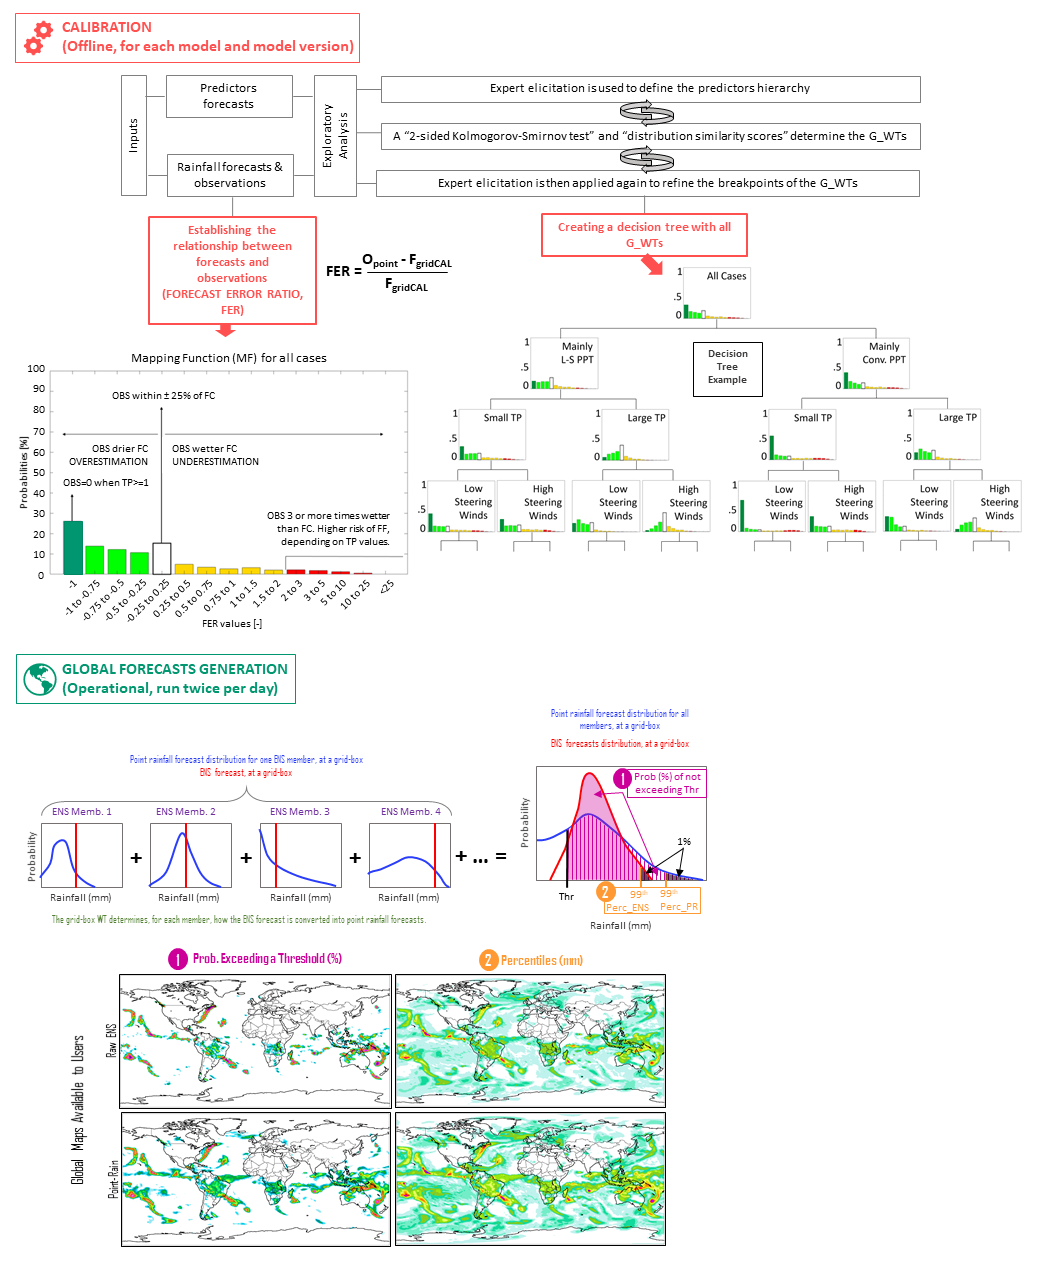
\includegraphics[width=53pc]{manuscript/Figures/ecPoint_Methodology.png}}
\caption{ecPoint Workflow. The left (red) panel represents the ecPoint's offline calibration process. The right (green) panel represents the ecPoint's forecast generation process and the products that can be derived from the post-processing output. The variable "rainfall" was used in this figure two illustrate both processes, calibration and forecast generation, but they can be used to post-process also other variables, e.g. "temperature".}
\label{ecPoint_Methodology}
\end{sidewaysfigure*}

ecPoint is a statistical post-processing technique that provides probabilistic bias-corrected forecasts at point scale from ensemble or deterministic numerical weather prediction (NWP) model outputs. Different hydro-meteorological variables, from different NWP models, can potentially be post-processed using the ecPoint technique to create, what is known as, the "ecPoint Family". ecPoint-Rainfall is the branch of the family that produces rainfall forecasts that mirror rain gauge measurements \citep{Hewson2020a}. In this paper, the ecPoint-Rainfall forecasts are post-processed raw ECMWF ENS rainfall forecasts. It is worth noting that what described to the following also applies to other NWP models. \par
To explain the reasons why ecPoint-Rainfall and raw ECMWF ENS rainfall forecasts may differ, let us consider an ENS grid cell and radar-derived totals for a rainfall event. Let us considered that the grid cell average rainfall total is about 17mm, while the minimum and maximum rainfall amounts are about 2mm and 60mm, respectively. The following can be stated. First, a completely accurate ENS member forecast would predict 17mm. However, this would not give the user any idea on what could be the spatial variability, within the grid cell, of the local (i.e. point) rainfall amounts when a particular G\_WT occurs. This describes an issue of sub-grid variability within the model grid box. Secondly, a particular G\_WT might show that an ENS member tends, on average, to over-predict (or under-predict) the grid-box rainfall by 15\%, delivering a forecast of 20mm (or 14mm) instead of 17mm. This describes an issue of model bias at grid-scale. By anticipating the sub-grid variability within the grid-box and correcting for biases in the model at grid-scale, ecPoint-Rainfall provides probabilities of bias-corrected rainfall forecasts at a point within the grid-box. However, ecPoint-Rainfall does not say where that point is within the ENS grid-box. \par
The calibration dataset for ecPoint-Rainfall is built applying the new concept of "Remote Calibration" described in \citet{Hewson2020a}. Typically, traditional post-processing methods use observations from a particular site. Such an approach limits the size of the calibration dataset, and forces to wait for at least ~20 years to have a robust calibration dataset, which still might not contain (enough) extremes cases for the considered site. The "Remote Calibration" approach removes any location labels and, instead, generates calibration datasets for particular G\_WTs pulling observations from where, around the world, those G\_WTs occurred. This approach facilitates the generation of extensive training datasets to post-process rainfall, including extremes. Indeed, the sites where a certain G\_WT occurs relatively often build the calibration dataset also for those sites where the same G\_WT would generate extreme rainfall. To give an order of magnitude, in order to create a similar calibration dataset for a location with similar size of one generated with the Remote Calibration approach, one would need to wait from hundreds to thousands of years. It is essential to highlight that the error bars on forecasts for globally extreme rainfall events (e.g. tropical cyclones) will be inevitably larger than for "not globally" extremes due to a lack of events in the calibration dataset. \par
 ecPoint-Rainfall outperforms raw ECMWF ENS in predicting localised rainfall events, including extremes \citet{Hewson2020a}. \par
In practice, ecPoint produces 100 equally probable point rainfall realisations for each of the 51 ENS members and each grid-box. For each grid-box, such 5100 values are distilled down into 99 percentile fields (1,2,..99) being those the final ecPoint-Rainfall product. Outputs from ecPoint-Rainfall are produced at ECMWF twice per day (at 00 and 12 UTC), up to 10 days, for overlapping 12-hourly accumulation periods, namely (T+0,T+12), (T+6,T+18),...,(T+234,T+246).


%%%%%%%%%%%%%%%%%%%%
% Background
\section{Background}
\begin{figure*}
\centerline{\includegraphics[width=39pc]{manuscript/Figures/Background_Location_AnnualRainfall_H_CR.png}}
\caption{Firstly, the flowchart describes the experiment processes that follow in the two experiment phases (real-time and offline). Secondly, the flowchart describes who, between developers (red squares), testers (blue squares) and developers & testers (cyan squares), conducted the experiment processes. Finally, the flowchart describes the possible experiment outcomes.}
\label{Location_Annual_Rainfall_H_CR}
\end{figure*}


%%%%%%%%%%%%%%%%%%%%
% Methods
\section{Methods} 

\begin{figure}
\centerline{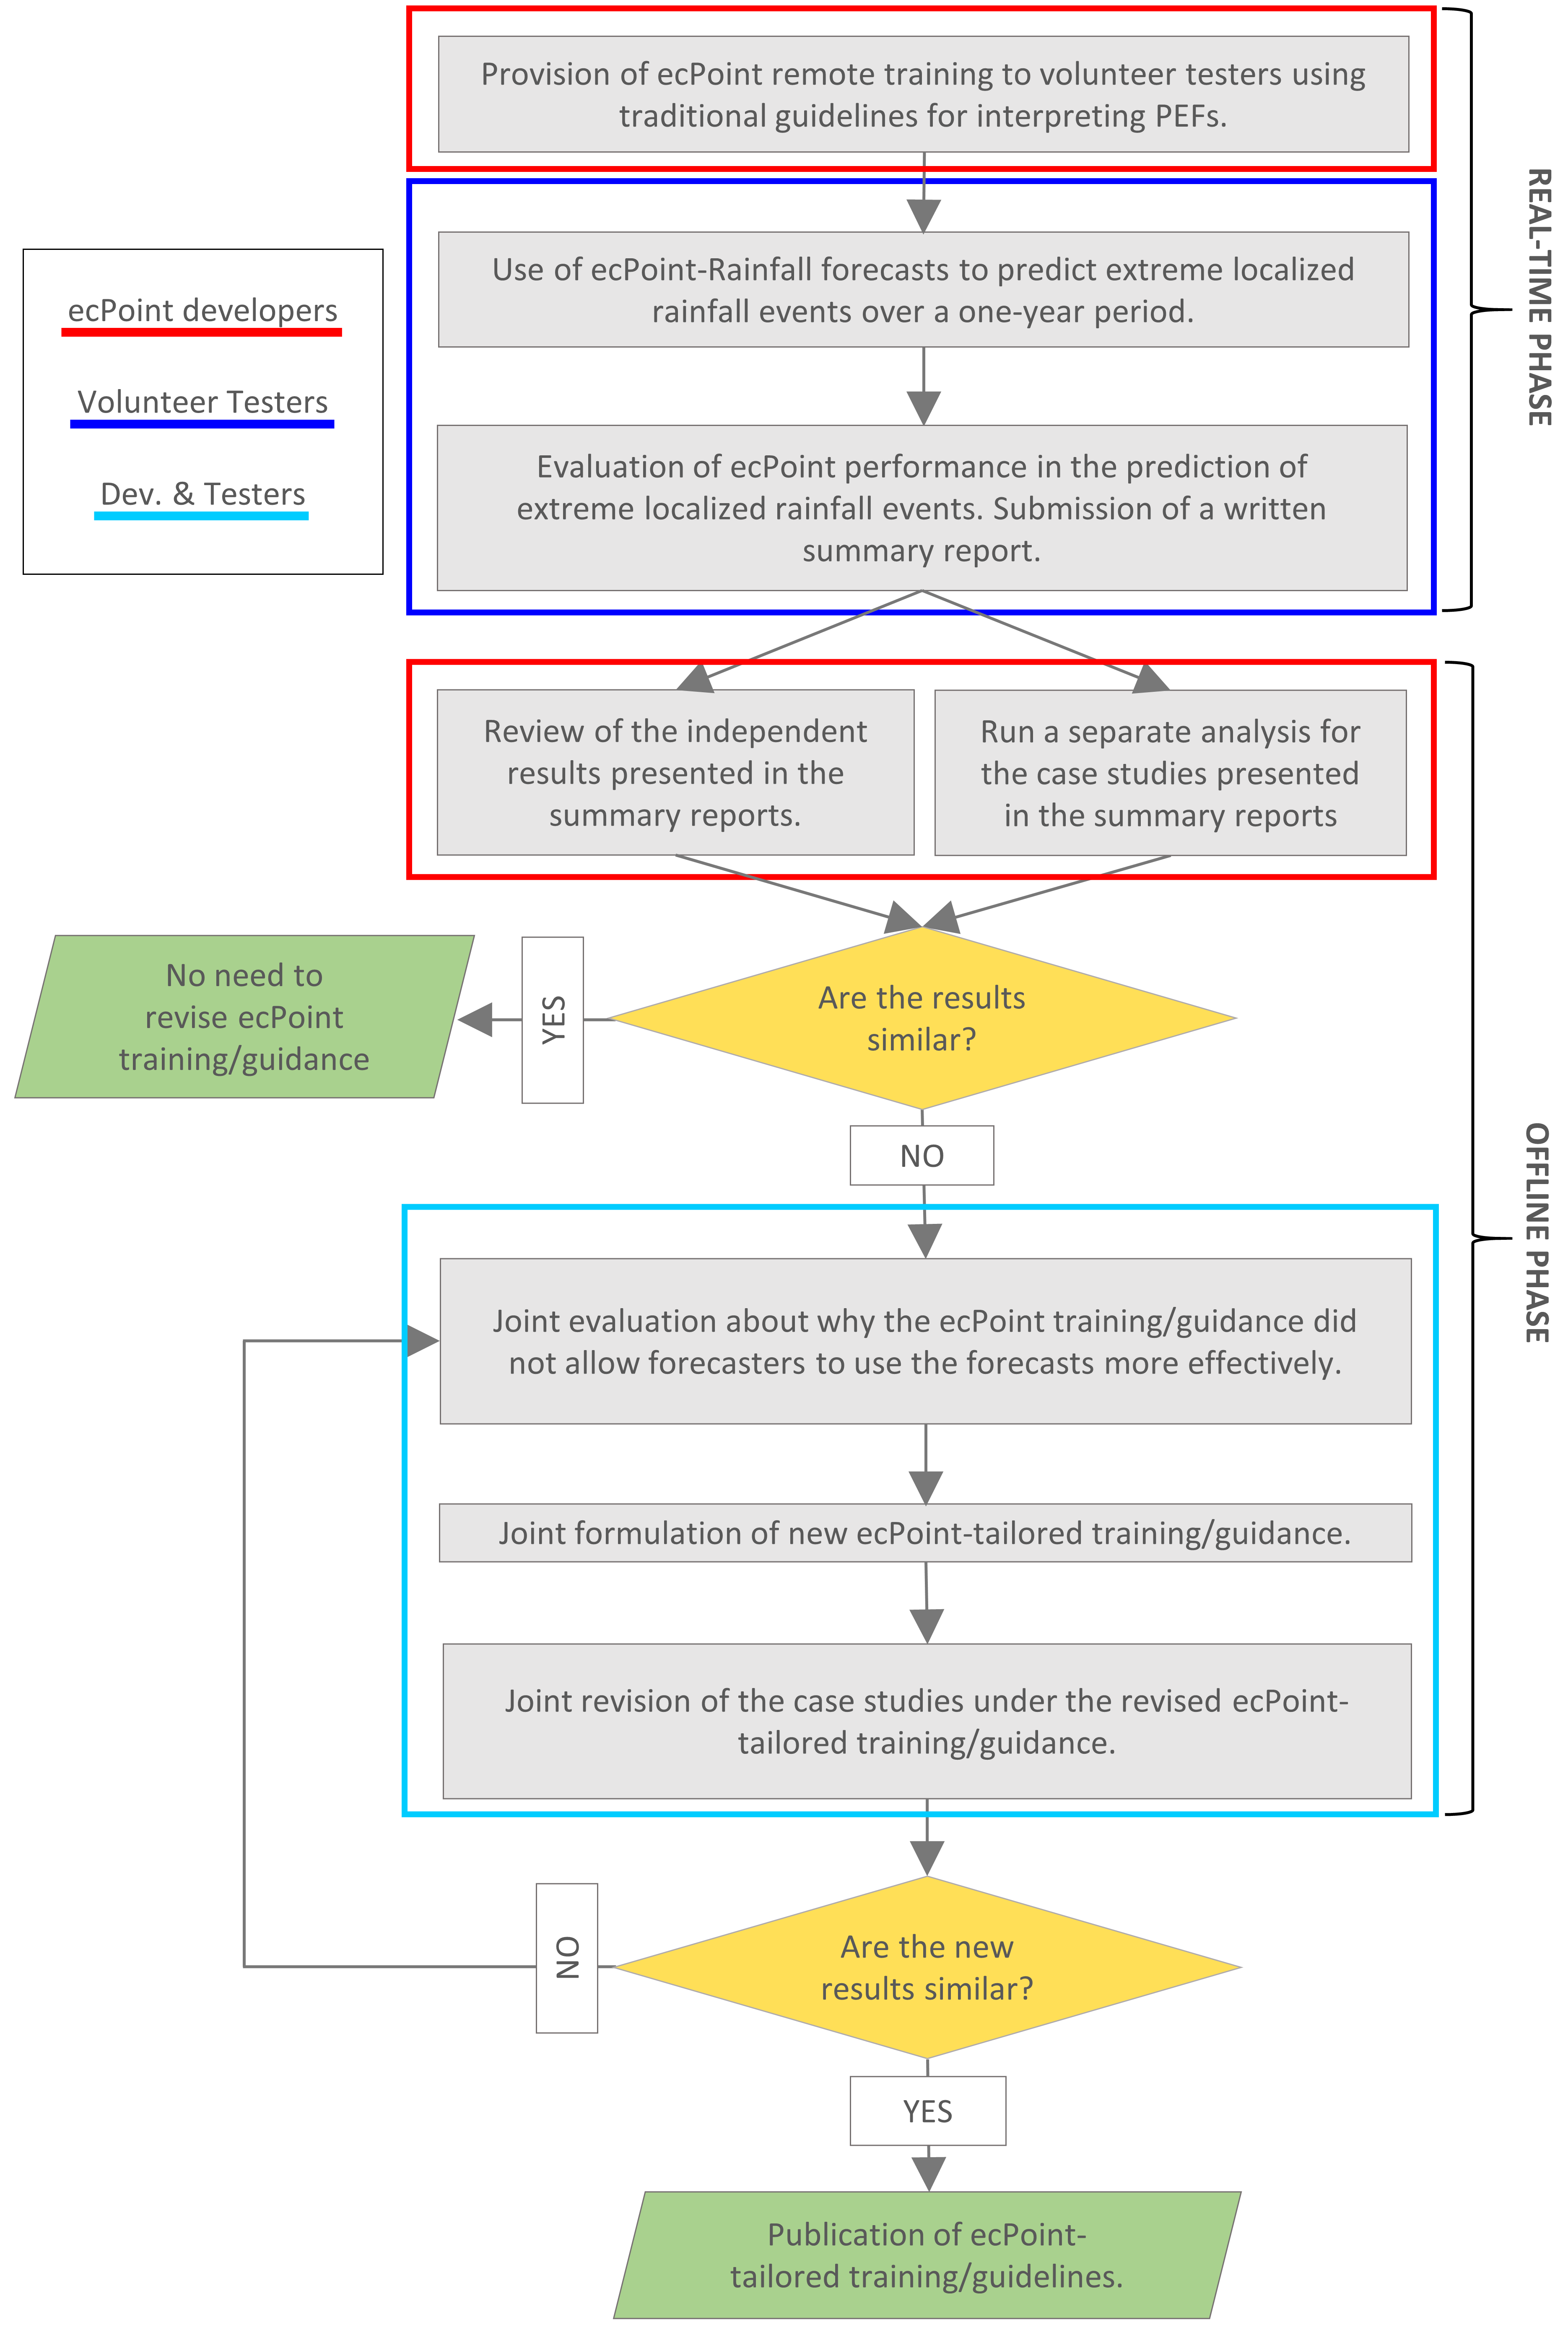
\includegraphics[width=19pc]{manuscript/Figures/Methods_FlowChart.png}}
\caption{Firstly, the flowchart describes the experiment processes that follow in the two experiment phases (real-time and offline). Secondly, the flowchart describes who, between developers (red squares), testers (blue squares) and developers & testers (cyan squares), conducted the experiment processes. Finally, the flowchart describes the possible experiment outcomes.}
\label{FlowChart}
\end{figure}

\begin{figure*}
\centerline{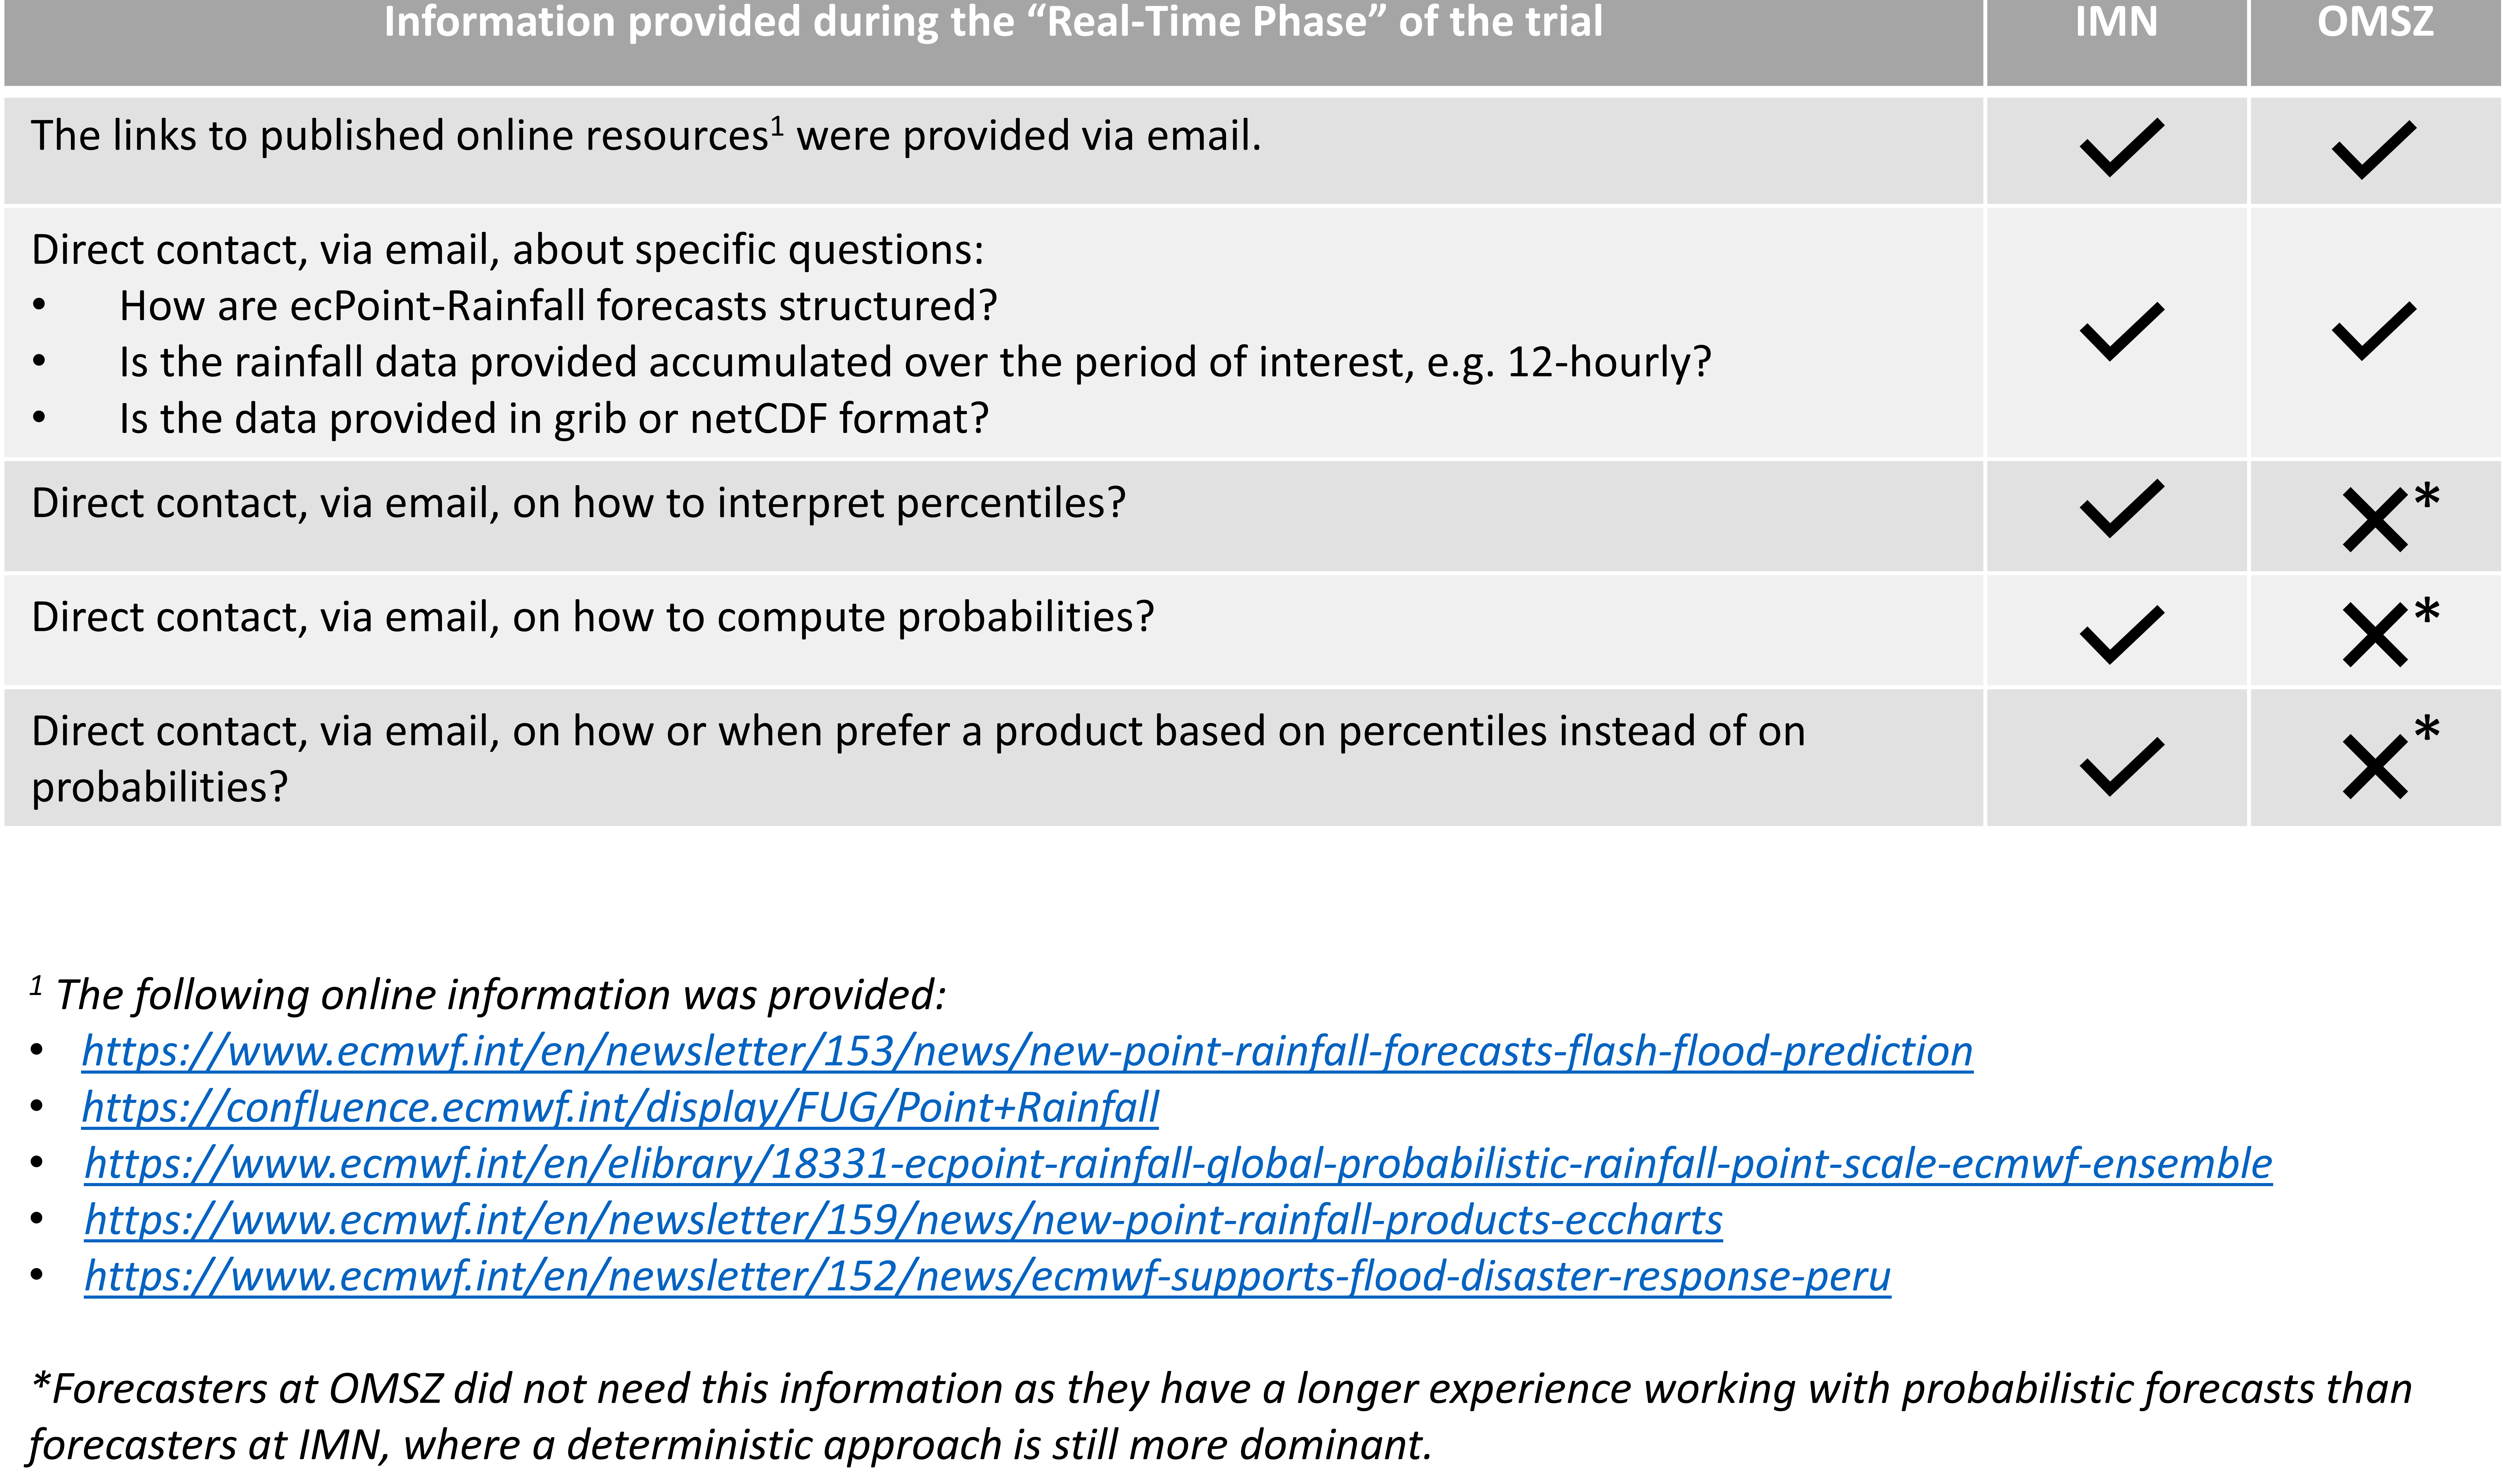
\includegraphics[width=39pc]{manuscript/Figures/Methods_Remote_Training.png}}
\caption{Training material provided to IMN and OMSZ at the beginning of the "Real-Time Phase" of the trial.}
\label{Remote_Training}
\end{figure*}
 
a.	Participants
Operational forecasters were chosen because their role of communicators has been widening in the recent years (citations).
Forecasters from Costa Rica and Hungary participated in the project. The sample is significantly diverse. OMSZ represents a NHMS in a country with continental climatology, and which possess extensive experience working with probabilistic forecasts. IMN represents a NHMS in a country with tropical climatology, and which possess a smaller experience working with probabilistic forecasts. 

b.	Experiment design
The aims of the project were:
•	Aim n.1: receive feedback on ecPoint-Rainfall performance. 
•	Aim n.2: receive feedback on its usefulness
The structure and the type of data analysis carried out in the experiment are described in the flowchart in Fig.3.

i.	“REAL-TIME” PHASE
To achieve aim n.1, a so called “real-time” phase was designed. At the beginning of this phase, a forecasters representative at the National Hydro-Met Service (NHMS) would receive remote training on ecPoint-Rainfall forecasts, to then pass the information to the other forecasters. Such remote training consisted, first, in sending via email the links to all the online training material on ecPoint-Rainfall produced prior the beginning of the trial (see the complete list in Table n.1). Upon request, a second stage in the remote training would have consisted in an exchange of emails or videocalls clarifying specific questions about the online training material. 
Whilst the remote training was taking place, the NHMSs started receiving via ftp the ecPoint-Rainfall forecasts up to day 10, twice per day (for runs at 0 and 12 UTC) over the domain set up for their respective countries (see Table 2 for the domain details). They would receive the ecPoint-Rainfall forecasts for an entire year, and quantitatively analyse its performance in predicting extreme localized rainfall in their respective countries. The decision was to base the quantitatively analysis on case studies due to a pragmatic reason. The volume of data available to participants (only one year of forecasts) was not particularly large. This made difficult other more systematic analysis (e.g. objective verification). Therefore, the findings of this phase make a smaller quantitative contribution to the more systematically verification carried out by Hewson and Pillosu (2020). However, the qualitative information that can be drawn from the local knowledge of the forecasters is extremely valuable to widen the knowledge of ecPoint developers in the definition of new parameters that could be used in the future post-processing developments.
The” real-time” phase was conducted between May 2018 - April 2019 for Costa Rica, and between July 2018 – June 2019. The “real-time phase” was conclude with both countries submitting an independent report about the ecPoint-Rainfall performance. Costa Rica and Hungary were left free in the choice of the case studies to analyse, the number of case studies to include in the report, and the analyses to carry out (e.g. run experiments with high resolution models to compare them with ecPoint-Rainfall, compare the new forecasts with the products that they normally use when predicting extreme localized rainfall, include in-situ observations, etc.). In this way, it would have been possible for the ecPoint developers to analyse (1) how ecPoint-Rainfall might be evaluated, and (2) how forecasters might incorporate ecPoint-Rainfall in their forecasting routines. However, both countries were asked to state at the end of the report what was their impression about ecPoint-Rainfall forecasts, replying to the following questions:
•	Was useful to have ecPoint-Rainfall, or was it only another just another product to add to the bulk of information already available at their NHMS? 
•	If adopted operationally, having ecPoint-Rainfall would have changed the forecasts for extreme localized rainfall created with their standard products?
The answers to these questions would have been the starting point for the conversations in the “offline” phase. 

ii.	“OFFLINE” PHASE
The “offline phase” started in April 2020. 
The “offline” phase was designed to collect information to achieve aim n.2. The information provided at the end of the independent report was the main object of discussion in this phase. A qualitative analysis was adopted in this phase. This choice was theoretically and practically driven. First, there was a commitment to seek to understand the perspectives about ecPoint-Rainfall of those being studied. Second, the collection of meaningful quantitative data was impossible due to the limited number of participants to the project. Yet, qualitative methods allowed us to collect rich qualitative data also to shed light to aspects that might limit the adoption of ecPoint-Rainfall forecasts in operational environments in future.
Structured or semi-structured interviews are commonly adopted to collect information about forecasters needs to improve predictions of high-impact weather (Wilson et al. 2019; Demuth et al. 2020), or collect information about their individual perspectives on the communication procedures for those forecasts (Joslyn et al. 2007; Joslyn et al. 2009; Joslyn and Savelli 2010; LeClerc and Joslyn 2015; Losee and Joslyn 2018; Doyle et al. 2019; Weyrich et al. 2019; Arnal et al. 2020; Emerton et al. 2020). However, for the goals of this study, best practice suggest that it would have been more appropriate to adopt in this phase a more informal discussion, approaching participants as fellow dialoguers rather than interviewers (Harding 2018). Indeed, this would have allowed ecPoint developers to put respondents at ease and not inhibited or constrained the respondents, obtaining in this way the sincerest answers about the performance of ecPoint-Rainfall (whatever they were, good or bad). Moreover, ecPoint developers were looking to identify with this study key themes which could be used in subsequent, more structured, interviews with future ecPoint users. 

All informal discussions were electronically conducted on each participant individually in turn. The first informal discussion was arranged as a videocall of one hour. Participants were then informed that if subsequent follow ups were needed, they would have been carried out primarily via email, but if they needed, videocall follow ups could have been arranged. 
The first informal discussion was guided by a list of open-ended questions that serve as a guide to elicit information from the respondents. They served as a start guide for the host (i.e. paper’s first author) to elicit information from the respondents during the conversation. This approach was adopted for its flexibility. Indeed, it allowed the conversation to start but, at the same time, allowed the conversation to follow its own path on what forecasters thought were the most important points were to highlight (on ecPoint-Rainfall performance, on how developers could improve the design of the product). That was an incredible source of information for ecPoint developers because they might have been aspects that were not anticipated by them. Indeed, this last aspect allowed as to include more questions or probes in the original list to be then asked or followed up with the other respondent. The original list of questions was developed collaboratively by ecPoint developers (Fatima Pillosu and Tim Hewson) based on questions raise during the reading of the final reports and ideas about how ecPoint-Rainfall forecasts could be developed. Such list was sent to the participants one week before the first videocall so they could prepare and feel more relaxed during the online conversation. The informal discussions began with broader objectives, asking background questions such as (1) what are the tools that they use to predict extreme localized rainfall, (1) how they make decisions when issuing forecasts in case of extreme localized rainfall, (2) what are their perceptions about global models’ performance in forecasting extreme localized rainfall in their countries, (3) what they think about the ability of post-processing to improve global NWP model guidance for extreme localized rainfall, and (4) examine context under which forecasters might take decisions on issuing or not alarms, (5) what is their degree of experience with probabilistic models and statistical post-processing, (6) provide background information about their core duties, (7) what are their forecast processes, including the synthesis of observational and model data used, (8) their ideas about needs to improve the prediction of extreme localized rainfall, (9) their process of  and the needs for communicating hazardous weather information with their partners. The interview guide is available in Table 1. Gradually, the questions moved to understand the level of proficiency with probabilistic forecasts. Eventually, questions focused on ecPoint-Rainfall, about its performance and an estimation of the level of goodness of the training material provided at the beginning of the project. Moreover, a series of not-planned topical probes were devised during the discussions and were used with the participants during follow ups to elicit further information from them. See Table 3 for a complete list of questions and (not-planned) topical probes. The results of this analysis are presented in section 5.1.
After the informal conversation were concluded, ecPoint developers collected information on how to develop ecPoint-Rainfall products that could have been more useful for each participant. Such products (e.g. combination map plots of probabilities exceeding an threshold and a specific percentile, CDFs, meteograms) were developed by ecPoint developers for the case studies included in the final reports, and presented via email to the respondents to see whether those products would have been more useful to their needs. This analysis is included in section 5.2
Finally, a thematic analysis (Harding 2018) was conducted to examine relationships or differences between the use that participants to the “ecPoint-Project” made of ecPoint-Rainfall forecasts on the basis of the guidelines provided. The results of this analysis are presented in section 5.3



%%%%%%%%%%%%%%%%%%%%
% Results
\section{Results}


%%%%%%%%%%%%%%%%%%%%
% Discussions
\section{Discussion}


%%%%%%%%%%%%%%%%%%%%
% Conclusions
\section{Conclusion}


%%%%%%%%%%%%%%%%%%%
% ACKNOWLEDGMENTS %
%%%%%%%%%%%%%%%%%%%
\acknowledgments


%%%%%%%%%%%%%%%%%%%%%%%%%%%%%%%
% DATA AVAILABILITY STATEMENT %
%%%%%%%%%%%%%%%%%%%%%%%%%%%%%%%
\datastatement
The data that support the findings of this study are available from the corresponding author upon request.


%%%%%%%%%%%%%%
% REFERENCES %
%%%%%%%%%%%%%%
\bibliographystyle{ametsoc2014}
\bibliography{references}

\end{document}